\documentclass[notes,11pt, aspectratio=169]{beamer}

\usepackage{pgfpages}
% These slides also contain speaker notes. You can print just the slides,
% just the notes, or both, depending on the setting below. Comment out the want
% you want.
\setbeameroption{hide notes} % Only slide
%\setbeameroption{show only notes} % Only notes
%\setbeameroption{show notes on second screen=right} % Both

\usepackage{helvet}
\usepackage[default]{lato}
\usepackage{array}



\usepackage{tikz}
\usepackage{verbatim}
\setbeamertemplate{note page}{\pagecolor{yellow!5}\insertnote}
\usetikzlibrary{positioning}
\usetikzlibrary{snakes}
\usetikzlibrary{calc}
\usetikzlibrary{arrows}
\usetikzlibrary{decorations.markings}
\usetikzlibrary{shapes.misc}
\usetikzlibrary{matrix,shapes,arrows,fit,tikzmark}
\usepackage{amsmath}
\usepackage{mathpazo}
\usepackage{hyperref}
\usepackage{lipsum}
\usepackage{multimedia}
\usepackage{graphicx}
\usepackage{multirow}
\usepackage{graphicx}
\usepackage{dcolumn}
\usepackage{bbm}
\newcolumntype{d}[0]{D{.}{.}{5}}
\usepackage{subfigure}

\usepackage{changepage}
\usepackage{appendixnumberbeamer}
\newcommand{\beginbackup}{
   \newcounter{framenumbervorappendix}
   \setcounter{framenumbervorappendix}{\value{framenumber}}
   \setbeamertemplate{footline}
   {
     \leavevmode%
     \hline
     box{%
       \begin{beamercolorbox}[wd=\paperwidth,ht=2.25ex,dp=1ex,right]{footlinecolor}%
%         \insertframenumber  \hspace*{2ex} 
       \end{beamercolorbox}}%
     \vskip0pt%
   }
 }
\newcommand{\backupend}{
   \addtocounter{framenumbervorappendix}{-\value{framenumber}}
   \addtocounter{framenumber}{\value{framenumbervorappendix}} 
}


\usepackage{graphicx}
\usepackage[space]{grffile}
\usepackage{booktabs}

% These are my colors -- there are many like them, but these ones are mine.
\definecolor{sage}{RGB}{102,153,102}
\definecolor{yellow}{RGB}{255,173,1}
\definecolor{purple}{RGB}{153,102,153}


\hypersetup{
  colorlinks=false,
  linkbordercolor = {white},
  linkcolor = {sage}
}


%% I use a beige off white for my background
\definecolor{MyBackground}{RGB}{255,253,218}

%% Uncomment this if you want to change the background color to something else
%\setbeamercolor{background canvas}{bg=MyBackground}

%% Change the bg color to adjust your transition slide background color!
\newenvironment{transitionframe}{
  \setbeamercolor{background canvas}{bg=white}
  \begin{frame}}{
    \end{frame}
}

\setbeamercolor{frametitle}{fg=sage}
\setbeamercolor{title}{fg=sage}
\setbeamertemplate{footline}[frame number]
\setbeamertemplate{navigation symbols}{} 
\setbeamertemplate{itemize items}{$\rightarrow$}
\setbeamercolor{itemize item}{fg=sage}
\setbeamercolor{itemize subitem}{fg=sage}
\setbeamercolor{enumerate item}{fg=sage}
\setbeamercolor{enumerate subitem}{fg=sage}
\setbeamercolor{button}{bg=MyBackground,fg=purple,}



% If you like road maps, rather than having clutter at the top, have a roadmap show up at the end of each section 
% (and after your introduction)
% Uncomment this is if you want the roadmap!
\AtBeginSection[]
{
   \begin{frame}
       \frametitle{Roadmap of Talk}
       \tableofcontents[currentsection]
   \end{frame}
}
\setbeamercolor{section in toc}{fg=sage}
\setbeamercolor{subsection in toc}{fg=sage}
\setbeamersize{text margin left=1em,text margin right=1em} 

\newenvironment{wideitemize}{\itemize\addtolength{\itemsep}{10pt}}{\enditemize}

\usepackage{environ}
\NewEnviron{videoframe}[1]{
  \begin{frame}
    \vspace{-8pt}
    \begin{columns}[onlytextwidth, T] % align columns
      \begin{column}{.58\textwidth}
        \begin{minipage}[t][\textheight][t]
          {\dimexpr\textwidth}
          \vspace{8pt}
          \hspace{4pt} {\Large \sc \textcolor{blue}{#1}}
          \vspace{8pt}
          
          \BODY
        \end{minipage}
      \end{column}%
      \hfill%
      \begin{column}{.42\textwidth}
        \colorbox{green!20}{\begin{minipage}[t][1.2\textheight][t]
            {\dimexpr\textwidth}
            Face goes here
          \end{minipage}}
      \end{column}%
    \end{columns}
  \end{frame}
}

\title[]{\textcolor{sage}{Labor Markets and Technological Change}}
\subtitle[]{Evidence from Electronic Health Records}
\author[]{Hanna Glenn\\PhD Candidate\\Emory University\\hanna.glenn@emory.edu}

\date{\today}


\begin{document}

%%% TIKZ STUFF
\tikzstyle{bigcirc} = [circle, minimum width=3cm, minimum height=1cm,text centered, draw=black, fill=sage!30]
\tikzstyle{medcirc} = [circle, minimum width=2.5cm, minimum height=1cm,text centered, draw=black, fill=sage!30]
\tikzstyle{smallcirc} = [circle, minimum width=2cm, minimum height=1cm,text centered, draw=black, fill=sage!30]
\tikzstyle{rect} = [rectangle, minimum width=3cm, minimum height=1cm, text centered, draw=black, fill=purple!30]
\tikzstyle{text} = [rectangle, minimum width=2cm, minimum height=1cm, text centered, draw=black, fill=green!100]
\tikzstyle{invisible} = [rectangle, minimum width=.001cm, minimum height=.001cm, text centered, draw=black!0, fill=red!0]
\tikzstyle{arrow} = [thick,->,>=stealth]
%%%% END TIKZ STUFF

% Title Slide
\begin{frame}
\maketitle
\end{frame}

\begin{frame}{Technology in Health Care}
    \centering
    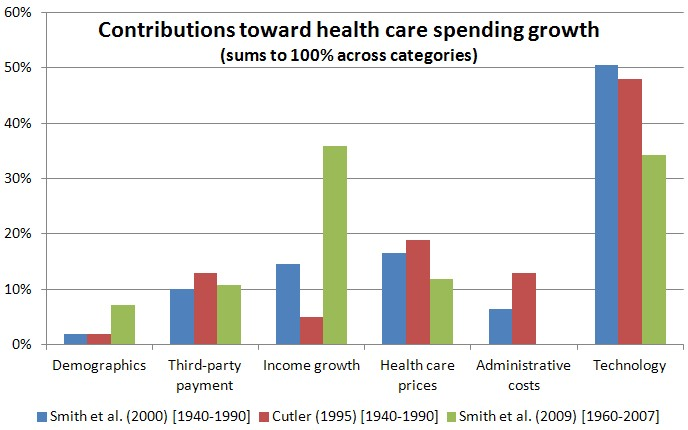
\includegraphics[scale=.4]{Objects/tech_graphic.jpg}
    
    \tiny{Source: \hyperlink{https://academyhealth.org/blog/2015-01/how-coverage-and-technology-interact}{https://academyhealth.org/blog/2015-01/how-coverage-and-technology-interact}}
    
\end{frame}

\begin{frame}{Electronic Health Records}
    \centering
    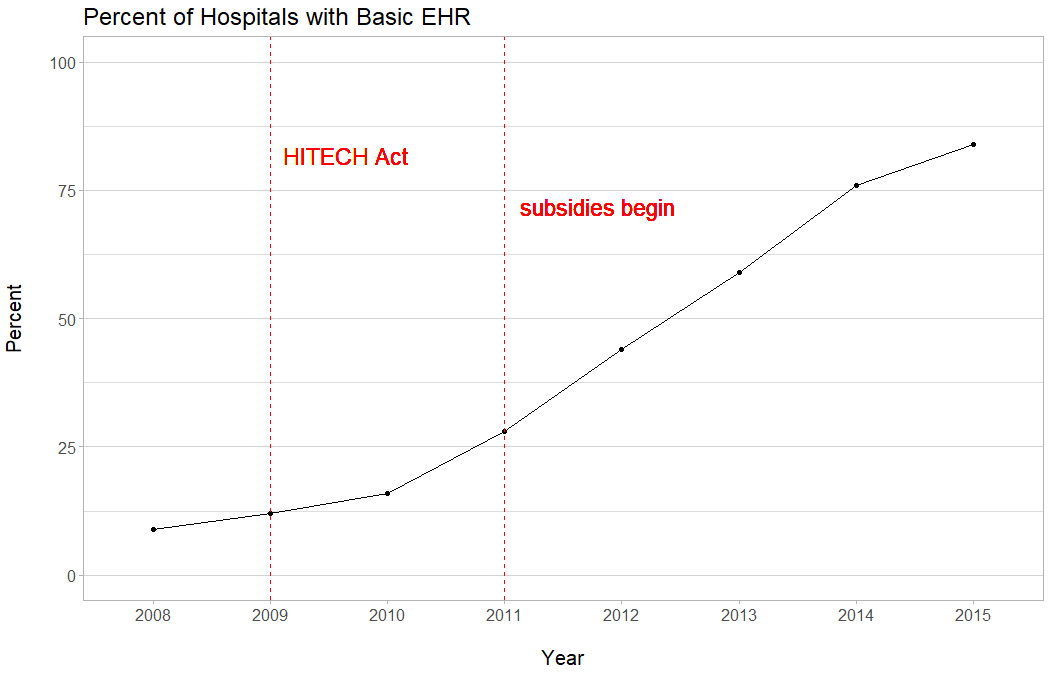
\includegraphics[scale=.4]{Objects/EHR_adoption_graph.PNG}
    
    \tiny{Source (data points): \hyperlink{https://www.healthit.gov/data/quickstats/non-federal-acute-care-hospital-electronic-health-record-adoption}{https://www.healthit.gov/data/quickstats/non-federal-acute-care-hospital-electronic-health-record-adoption}}
\end{frame}

\begin{frame}[fragile]{What is an Electronic Health Record (EHR)?}
Health information stored digitally in a software
                \vspace{2mm}
\begin{center}
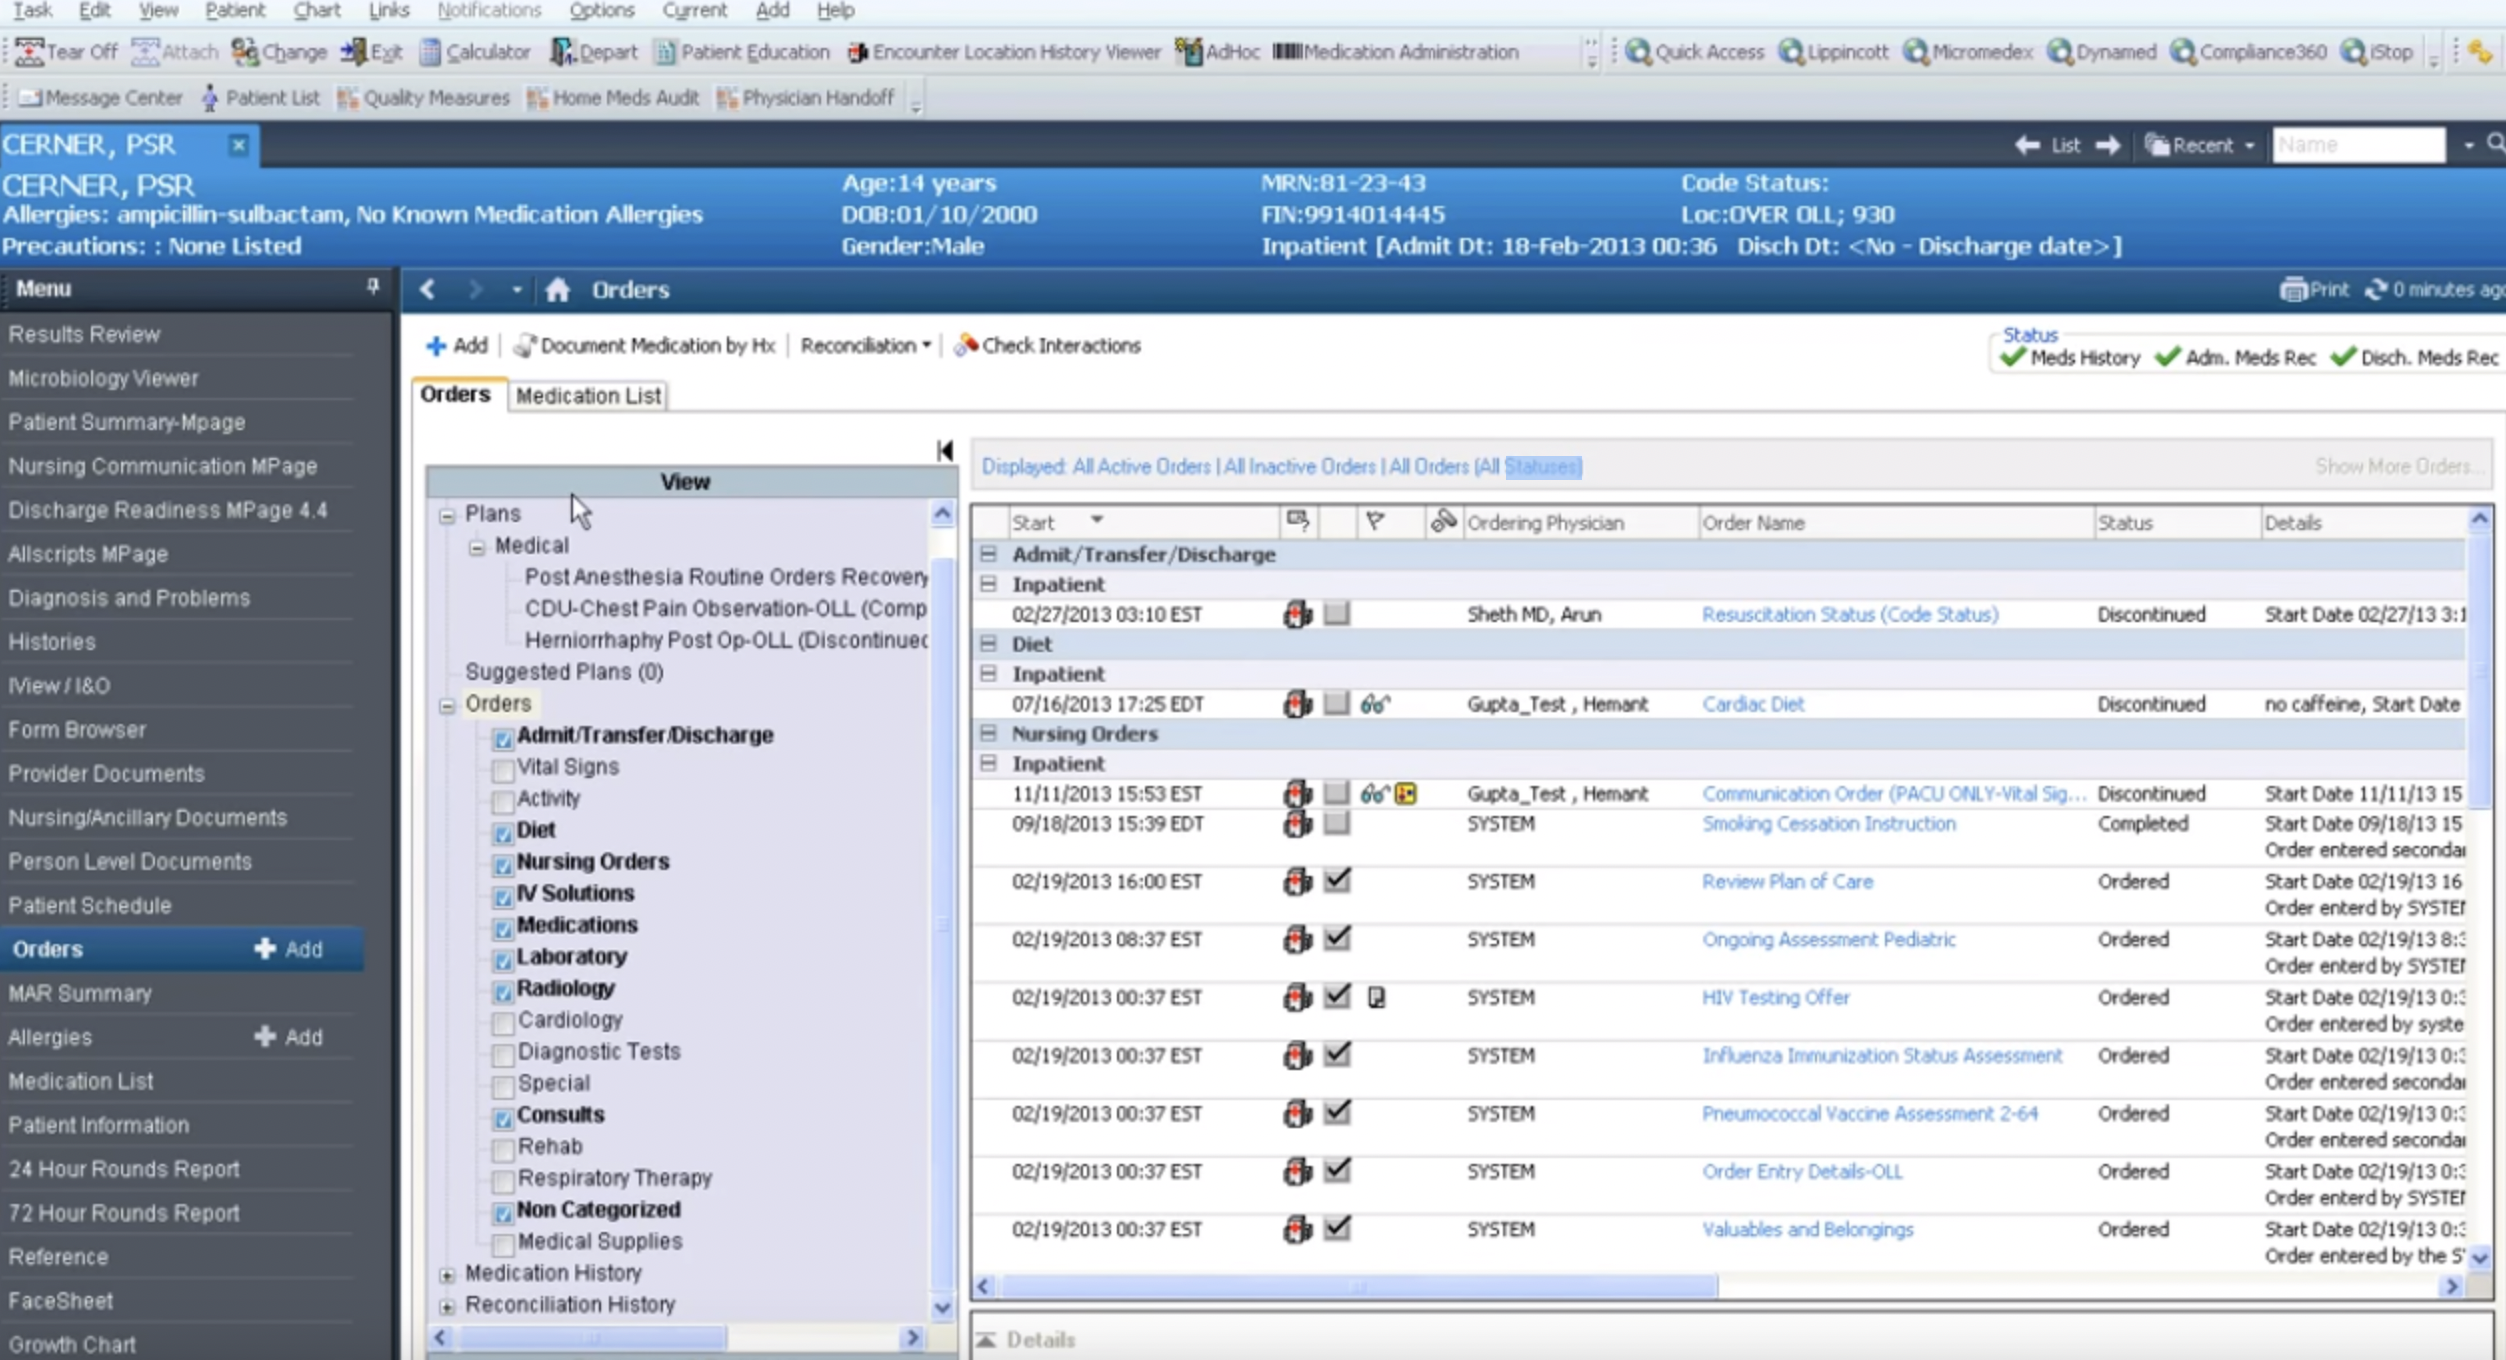
\includegraphics[scale=.25]{Objects/cernerscreenshot.png}

\tiny{Source: \hyperlink{https://softwareconnect.com/ehr/epic/}{https://softwareconnect.com/ehr/epic/}}
\vspace{-4mm}
\end{center}
\end{frame}


\begin{frame}{What we know about EHRs already}
Quality of Care:
\begin{itemize}
    \item Haven't seen the improvements expected for median patients
    \item \scriptsize Buntin et al. (2011), Agha (2014), Freedman et al. (2015), McCullough et al. (2016), Meyerhoefer et al. (2016)
\end{itemize}

\vspace{6mm}

Cost and Efficiency:
\begin{itemize}
    \item Maybe some gains, but not in all cases
    \item \scriptsize Agha (2014), Dranove et al. (2014), Hitt \& Tambe (2016)
\end{itemize}

\vspace{6mm}

Productivity:
\begin{itemize}
    \item Depends on the setting, positive effects are small
    \item \scriptsize McCullough et al. (2013), Hitt \& Tambe (2016), Meyerhoefer et al. (2016)
\end{itemize}    

\vspace{3mm}
\pause
\textcolor{purple}{this paper: \underline{Did EHR adoption in hospitals affect labor market behaviors of physicians in hospitals?}}
\end{frame}



\begin{frame}{Physician Response to EHRs}
\centering

\includegraphics[scale=.45]{Objects/EHR tweet.PNG}
\end{frame}

\begin{frame}{Physician Response to EHRs}
\centering

\includegraphics[scale=.5]{Objects/News Clip3.PNG}
\end{frame}

\begin{frame}{This Paper}
Did EHR implementation in hospitals affect labor market decisions of hospitalists?

\vspace{5mm}
\centering
\begin{tikzpicture}[node distance=2cm]
\node (inv1) [invisible] {};
\node (bigcirc) [bigcirc, left of=inv1, xshift=.5cm, yshift=.13cm] {Hospitalists: $\mathbbm{H}$};
\node (rect) [rect, below of=bigcirc, yshift=-.5cm] {EHR in Hospital};

\node (inv2) [invisible, right of=inv1, xshift=2.5cm] {};
\node (medcirc) [medcirc, left of=inv2, xshift=.7cm, yshift=.13cm] {$\mathbbm{H}\backslash\mathbbm{E}$};

\node (inv3) [invisible, right of=inv2, xshift=2.5cm] {};
\node (smallcirc) [smallcirc, left of=inv3, xshift=.4cm, yshift=.13cm]{$\mathbbm{H}\backslash\mathbbm{(E\cup\mathbbm{O}})$};

\node  (retire) [text, above of=bigcirc, xshift=2.5cm, yshift=.3cm, align=center] {Exit Clinical Work:  $\mathbbm{E}$\\(Ext. Margin)};
\node  (office) [text, above of=medcirc, xshift=2.5cm, yshift=.3cm, align=center] {Switch Job Setting: $\mathbbm{O}$};
\node  (prod) [text, below of=smallcirc, align=center] {Productivity\\(Int. Margin)};

\draw [arrow] (rect) -- (bigcirc);
\draw [arrow] (bigcirc) -- (medcirc);
\draw [arrow] (medcirc) -- (smallcirc);
\draw [arrow] (inv1) -- (retire);
\draw [arrow] (inv2) -- (office);
\draw [arrow] (smallcirc) -- (prod);
\end{tikzpicture}
\end{frame}



\begin{frame}[fragile]{Data}
Panel of hospitalists from 2009-2017 with information on whether their hospital uses an EHR and various labor market outcomes\\
                \vspace{3mm}
\begin{wideitemize}
    \item MDPPAS data: physician specialty, aggregation of Medicare patients seen
    \item CMS Shared Patient Data: connect hospitals and physicians by the number of patients they share
    \item AHA Survey \& HIMSS: Hospital level EHR information
\end{wideitemize}
\end{frame}

\begin{frame}{Identification Strategy}
    Difference in differences:
    \begin{itemize}
        \item Use variation in timing of hospitals adopting EHRs, compare hospitalists before and after exposure to the EHR
    \end{itemize}
    
                \vspace{5mm}
                
    \underline{Key assumption}: Hospital implementing EHR is exogenous shock to hospitalist behavior. That is, hospitalists are not selecting into exposure to EHR
\end{frame}


\begin{frame}{Estimation}
Treatment: Exposure to EHR\\
                \vspace{4mm}
Staggered treatment timing, Callaway and Sant'Anna (2021) average group time treatment effects:
$$ATT(g,t)=\mathbbm{E}[Y_t(g)-Y_t(0)|G_g=1]$$

\vspace{-1mm}

\begin{wideitemize}
    \item Not-yet-treated units
    \item Aggregate to get familiar event study plot
\end{wideitemize}

\vspace{3mm}

\pause Assumptions:
\begin{enumerate}
    \item No reversal of treatment
    \item No anticipation of treatment (can be relaxed)
    \item Parallel trends
\end{enumerate} 
\end{frame}


\begin{frame}{EHRs and Exit}
Decision to no longer see patients is multidimensional: retirement? switching type of job?
                \vspace{2mm}
\begin{itemize}
    \item Retirement is thought of as a function of age and wealth, and can depend on shocks such as health or job loss\\ \scriptsize{Hall and Johnson (1980), Gordon and Blinder (1980), Hamermesh (1985)}
                \vspace{3mm}
                \normalsize
                
    \item On average, physicians plan to retire at age 60 but don't actually retire until age 69 \\ \scriptsize{Collier (2017)}
                \vspace{3mm}
                \normalsize
                
    \item 13\% of physicians are considering a career change\\ \scriptsize{Physicians Foundation (2016)}
                \normalsize

\end{itemize}

\vspace{5mm}
\textcolor{purple}{I measure this as no longer seeing Medicare patients\ (mean: 3\%)}
\end{frame}


\begin{frame}{Effect of EHR Exposure on Exit}
\label{Effect of EHR Exposure on Exit}
\begin{figure}[ht]
    \centering
    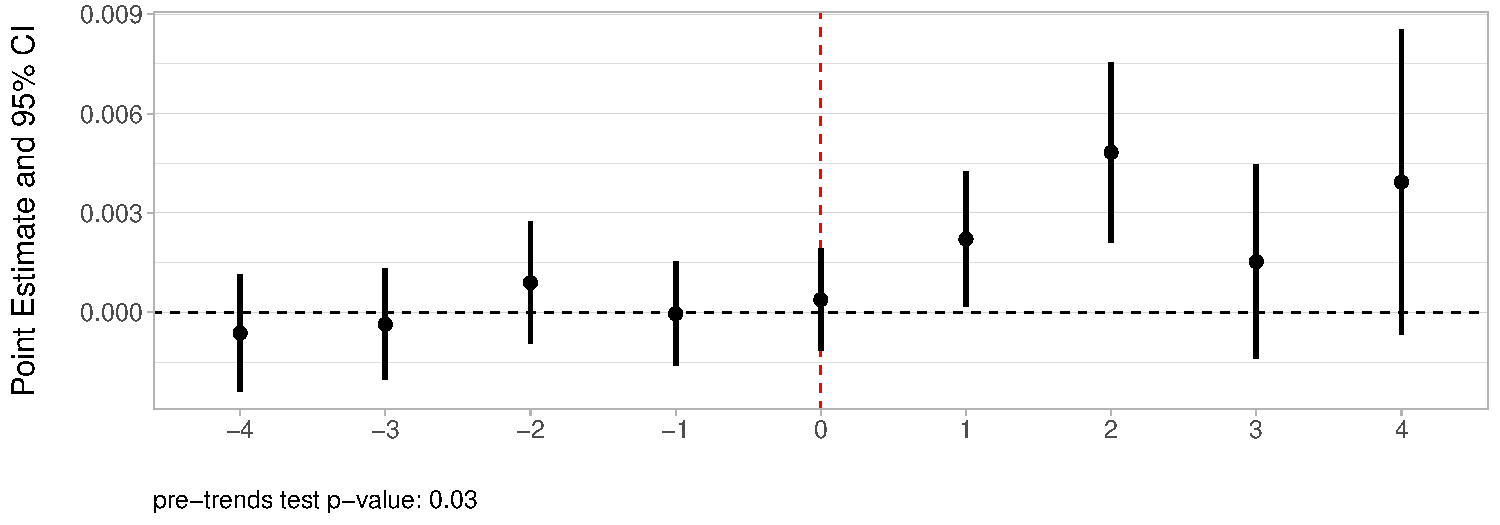
\includegraphics[scale=.5]{Objects/retire_plot_all.pdf}
\end{figure}
$\rightarrow$ 7\% and 15\% increase relative to the mean -- 100 additional hospitalists leaving

\hyperlink{Robustness: Retirement}{\beamerbutton{retire}}
\end{frame}

\begin{frame}{Effect of EHR Exposure on Exit: Age Groups}
\label{Effect of EHR Exposure on Retirement: Age Groups}
\begin{figure}[ht]
\centering
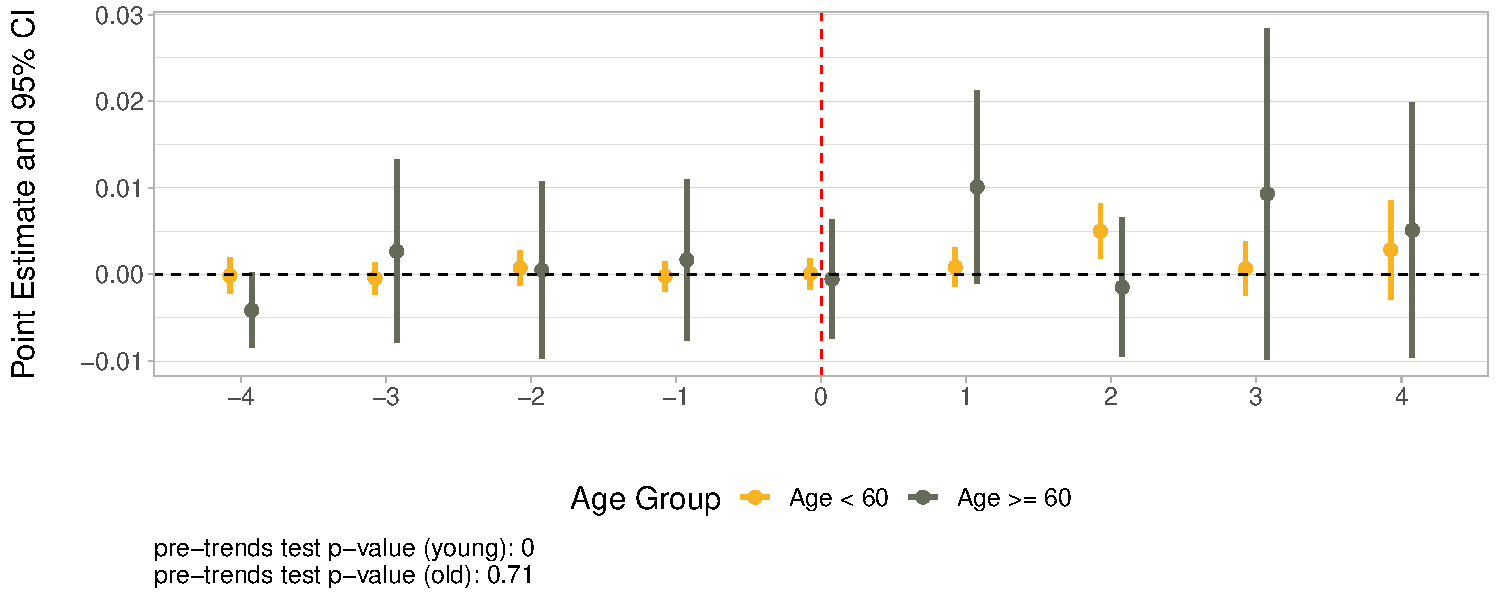
\includegraphics[scale=.5]{Objects/retire_plot_ages.pdf}
\end{figure}
\end{frame}


\begin{frame}{EHRs and Job Setting}
Most physicians will not be induced to exit because of EHRs
\begin{itemize}
    \item Another way to avoid (or be exposed to) new technology is to switch location of practice
                \vspace{3mm}
    \item Literature shows job switching is closely tied to job satisfaction\\ \scriptsize Aklerlof, Rose and Yellen (1988), Chadi and Hetschko (2017)
                \normalsize
    \end{itemize}

    \vspace{5mm}
    \textcolor{purple}{Measured as whether fraction of patients seen in office setting is $>$ 0 (mean: 28\%)}
\end{frame}

\begin{frame}{Effect of EHR Exposure on Likelihood of Working in Office}
\label{Effect of EHR Exposure on Likelihood of Working in Office}
\begin{figure}[ht]
    \centering
    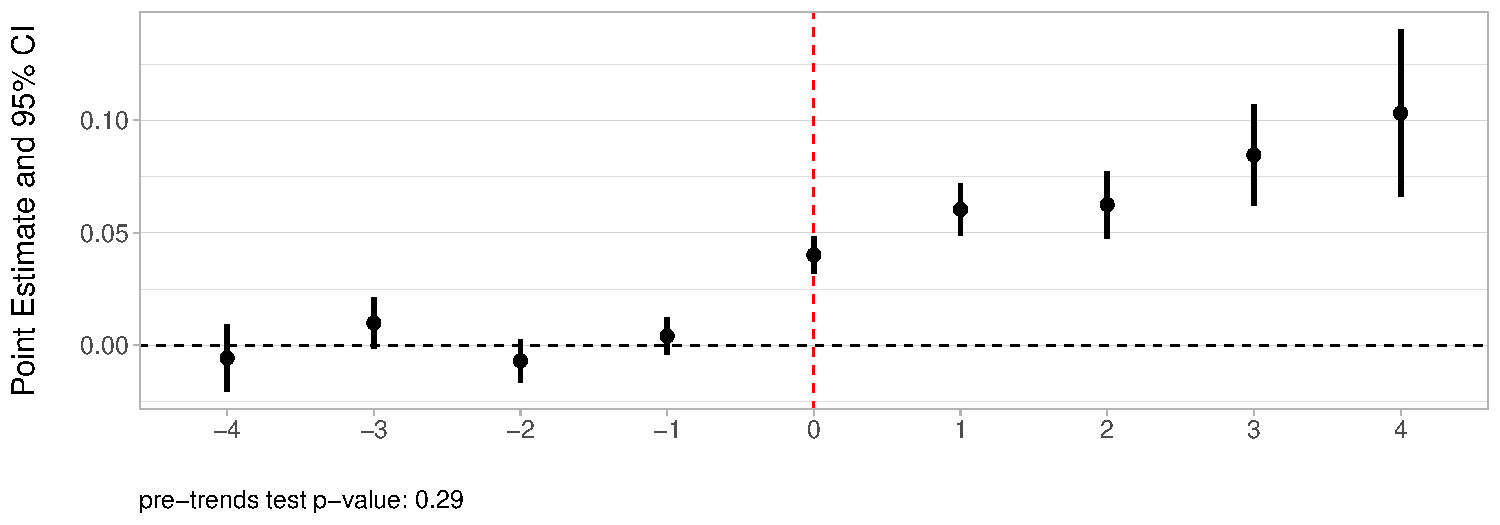
\includegraphics[scale=.5]{Objects/officeind_plot_all.pdf}
\end{figure}
$\rightarrow$ 15-38\% increase relative to the mean -- roughly 1-2,000 physicians who start seeing patients in an office\\
$\rightarrow$ Similar for both age groups

\hyperlink{Robustness: Indicator for Working in Office}{\beamerbutton{office ind.}}
\end{frame}



\begin{frame}{EHRs and Productivity}
Past research on information technology: productivity typically increases \\ \scriptsize (Brynjolfsson and Hitt 2003; Bartel, Ichniowski and Shaw 2007; Bloom, Sadun, and Reenen 2012b)
                \vspace{6mm}
                \normalsize 
                
We can see how productivity is affected for hospitalists who stay in the same hospital after exposure to EHR
                \vspace{3mm}
\begin{itemize}
    \item Expected effect is ambiguous
\end{itemize}

\vspace{5mm}
\textcolor{purple}{Measured as number of Medicare patients seen (mean: 325)}
\end{frame}

\begin{frame}{Effect of EHR Exposure on Patient Count}
\label{Effect of EHR Exposure on Patient Count}
\label{Results: Patient Count}
\begin{figure}[ht]
\centering
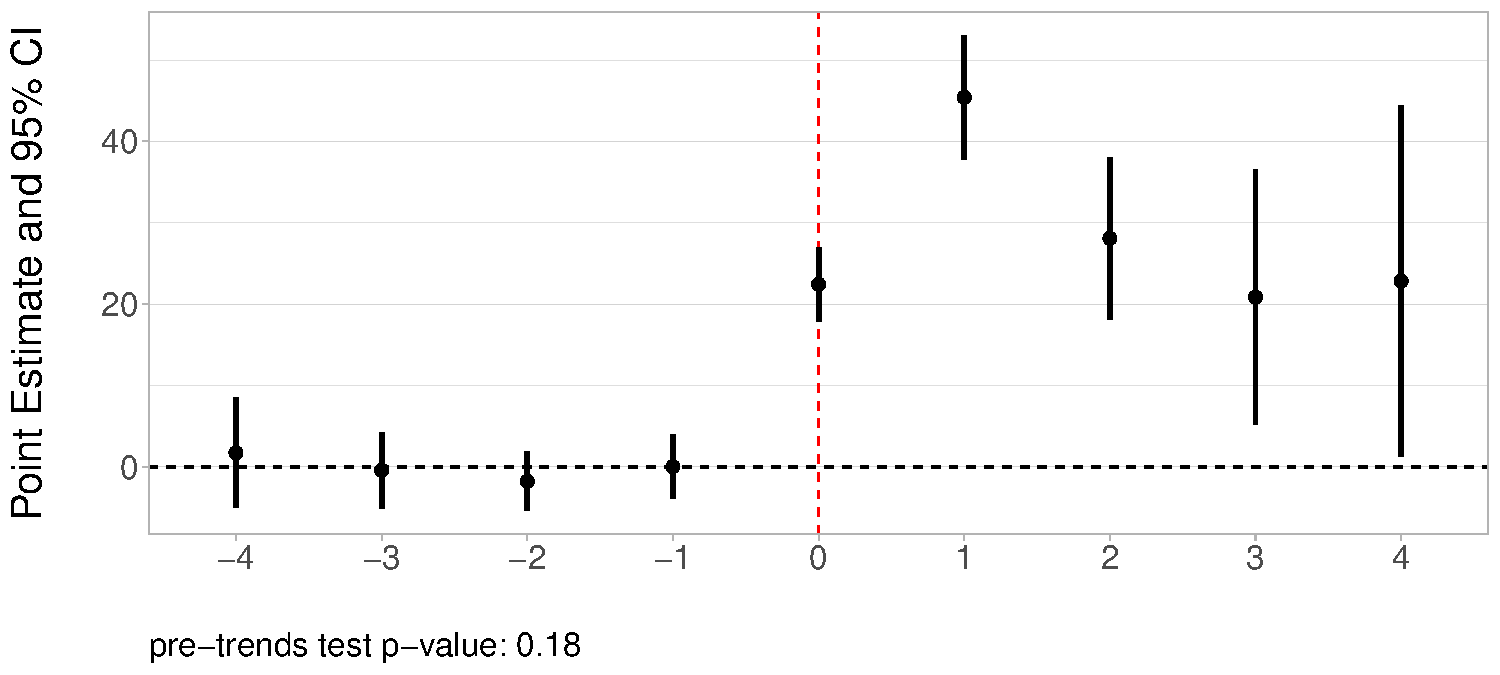
\includegraphics[scale=.5]{Objects/patient_plot_all.pdf}
\end{figure}
$\rightarrow$ 6-14\% increase relative to the mean\\ \hyperlink{patient count broken down by group}{\beamerbutton{groups}}

\hyperlink{Robustness: Patient Count}{\beamerbutton{patient count}}
\end{frame}



\begin{frame}{Summary and Implications}

\underline{Summary:} Hospitalists change labor market behavior as a result of technology change in work environment

                \vspace{5mm}

\underline{Implications}: 
\begin{itemize}
\item Unintended consequences of a policy leading to rapid technology adoption
\item Access to care
\item potentially has downstream affects for patient outcomes
\end{itemize}
\end{frame}

\begin{frame}{}
    \centering
    Thank you! \\
    hanna.glenn@emory.edu
\end{frame}

\begin{frame}[noframenumbering, label=ch1robustness]{Robustness}
\label{Robustness}
\begin{enumerate}
    \item Limiting years and using never-treated as control
            \vspace{3mm}
    \item Anticipation
            \vspace{3mm}
    \item Parallel trends
            \vspace{3mm}
    \item Other estimators
    \vspace{5mm}
    

\hyperlink{Lee (2009) Bounds}{\beamerbutton{Lee (2009) bounds}}
\hyperlink{TWFE}{\beamerbutton{TWFE}}
\hyperlink{Other Estimators for Staggered Treatment}{\beamerbutton{Estimators}}
\end{enumerate}
\end{frame}


% JUMP SLIDES! %%%%%%%%%%%%%%%%%%%%%%%%%%%%%%%%%%%%%%%%%%%%%%%%%%%%%%%%%%%%%%%%%%
%%%%%%%%%%%%%%%%%%%%%%%%%%%%%%%%%%%%%%%%%%%%%%%%%%%%%%%%%%%%%%%%%%%%%%%%%%%%%%%%%%
%%%%%%%%%%%%%%%%%%%%%%%%%%%%%%%%%%%%%%%%%%%%%%%%%%%%%%%%%%%%%%%%%%%%%%%%%%%%%%%%%

% first chapter jump slides %

\begin{frame}[noframenumbering]{Patient Count Broken Down by Group}
\label{patient count broken down by group}
\centering
    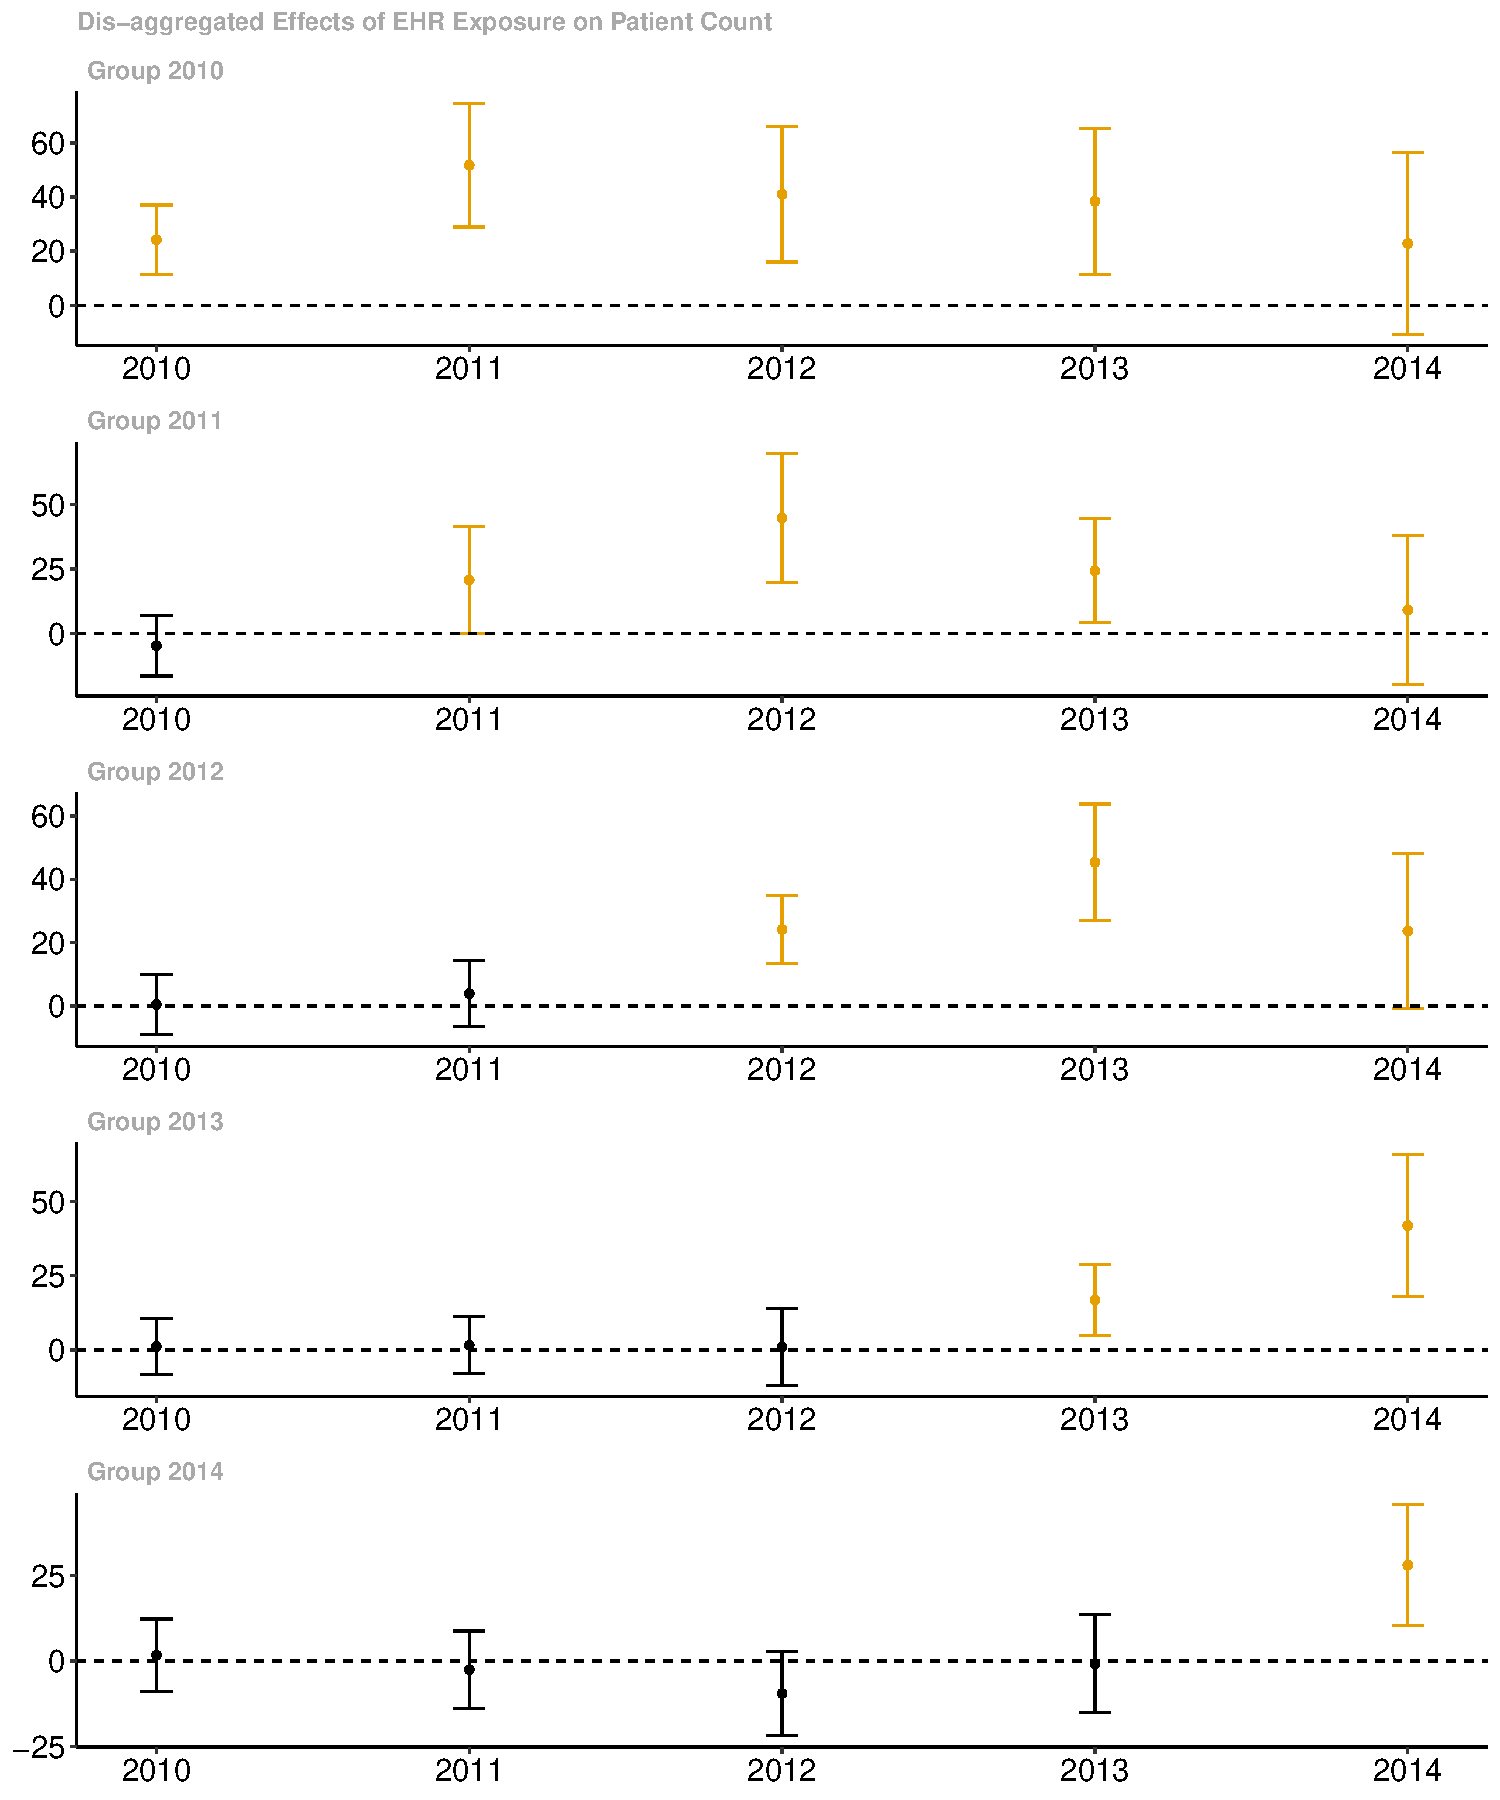
\includegraphics[scale=.25]{Objects/patient_group.pdf}
\hyperlink{Results: Patient Count}{\beamerbutton{back}}
\end{frame}

\begin{frame}[noframenumbering]{Lee (2009) Bounds}
\label{Lee (2009) Bounds}
    EHR exposure affects whether physicians are included in the analysis (since I drop those who retire or move), indicating a nonrandom attrition problem for productivity analysis.
    \begin{itemize}
        \item 18\% dropped in control group
        \item 36\% dropped in treatment group 
    \end{itemize}
    Monotonicity $\rightarrow$ EHR exposure increases the likelihood of retiring or moving workplace settings and no physicians remain in the sample under treatment who would have retired or moved in the absence of EHR exposure
    
    \begin{itemize}
        \item Patient count $\in$ (55,125)
        \hyperlink{Robustness}{\beamerbutton{back}}
    \end{itemize}
\end{frame}

\begin{frame}[noframenumbering]{Robustness: Exit}
\label{Robustness: Retirement}
\centering
    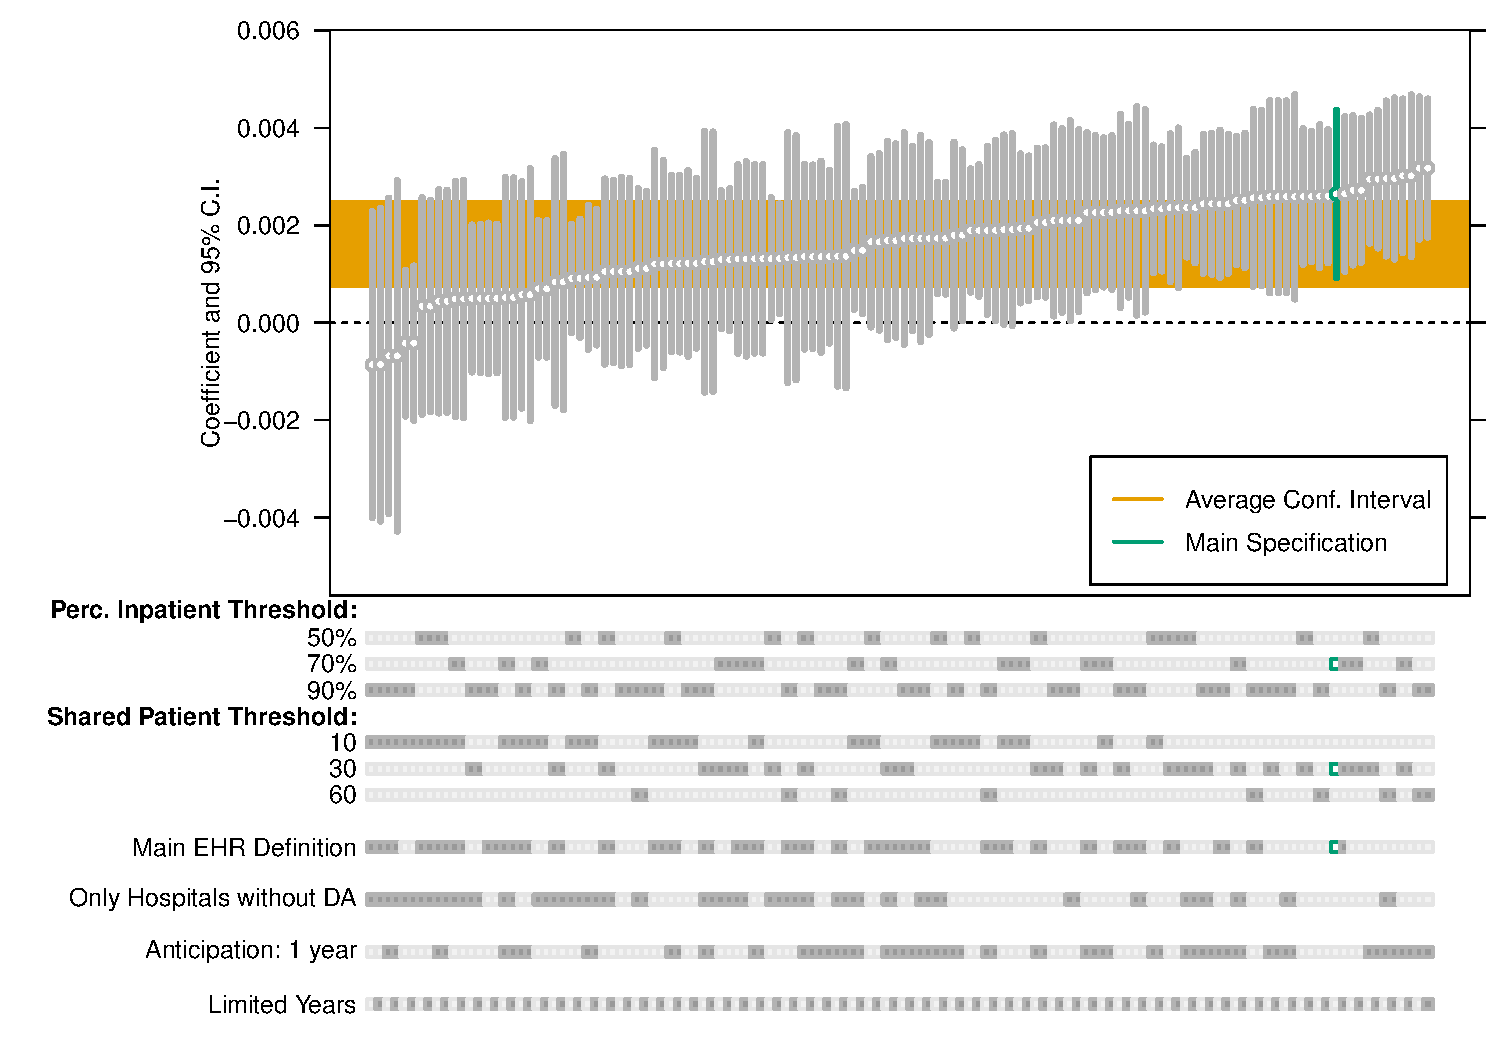
\includegraphics[scale=.5]{Objects/retire_chart.pdf}
    \hyperlink{Effect of EHR Exposure on Exit}{\beamerbutton{back}}
\end{frame}

\begin{frame}[noframenumbering]{Robustness: Indicator for Working in Office}
\label{Robustness: Indicator for Working in Office}
\centering
    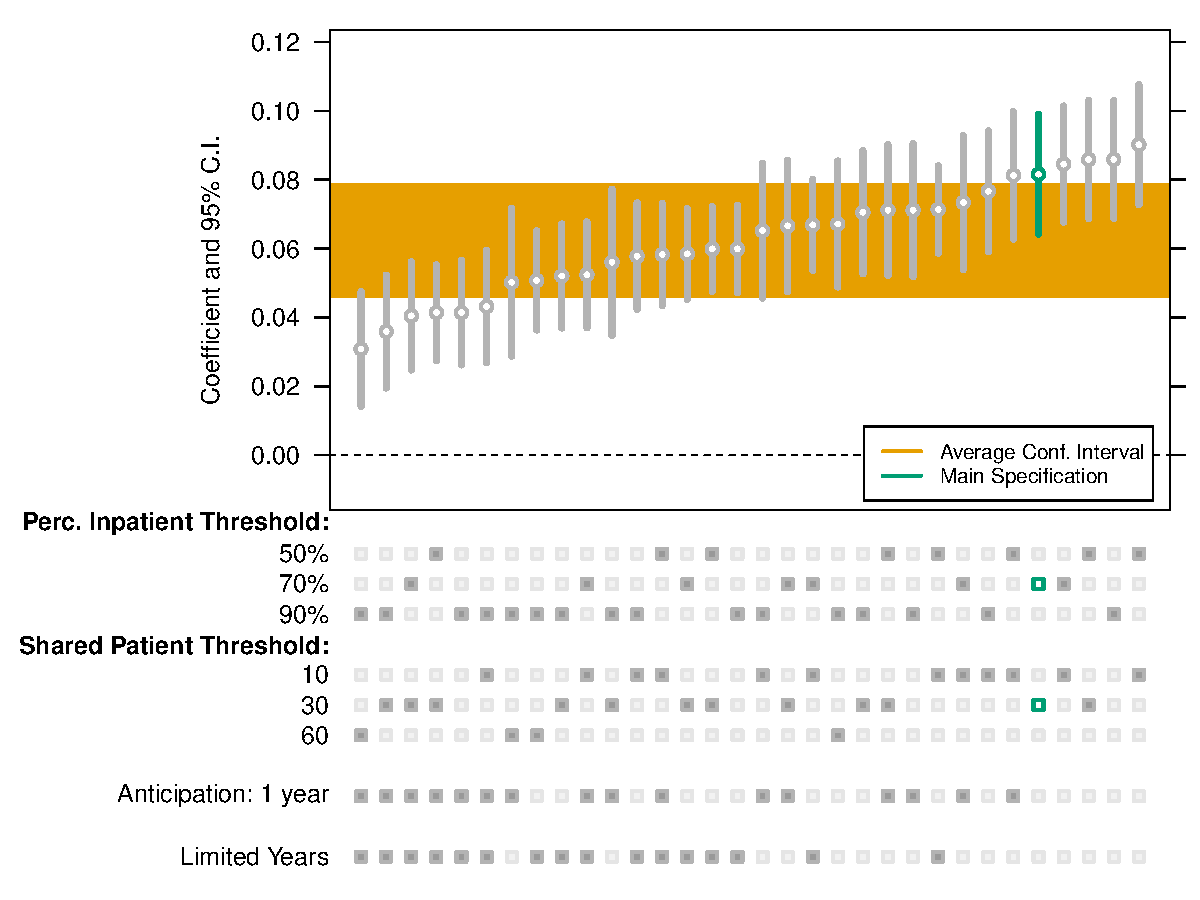
\includegraphics[scale=.45]{Objects/office_ind_chart.pdf}
    \hyperlink{Effect of EHR Exposure on Likelihood of Working in Office}{\beamerbutton{back}}
\end{frame}

\begin{frame}[noframenumbering]{Robustness: Frac. Patients in Office}
\label{Robustness: Frac. Patients in Office}
\centering
    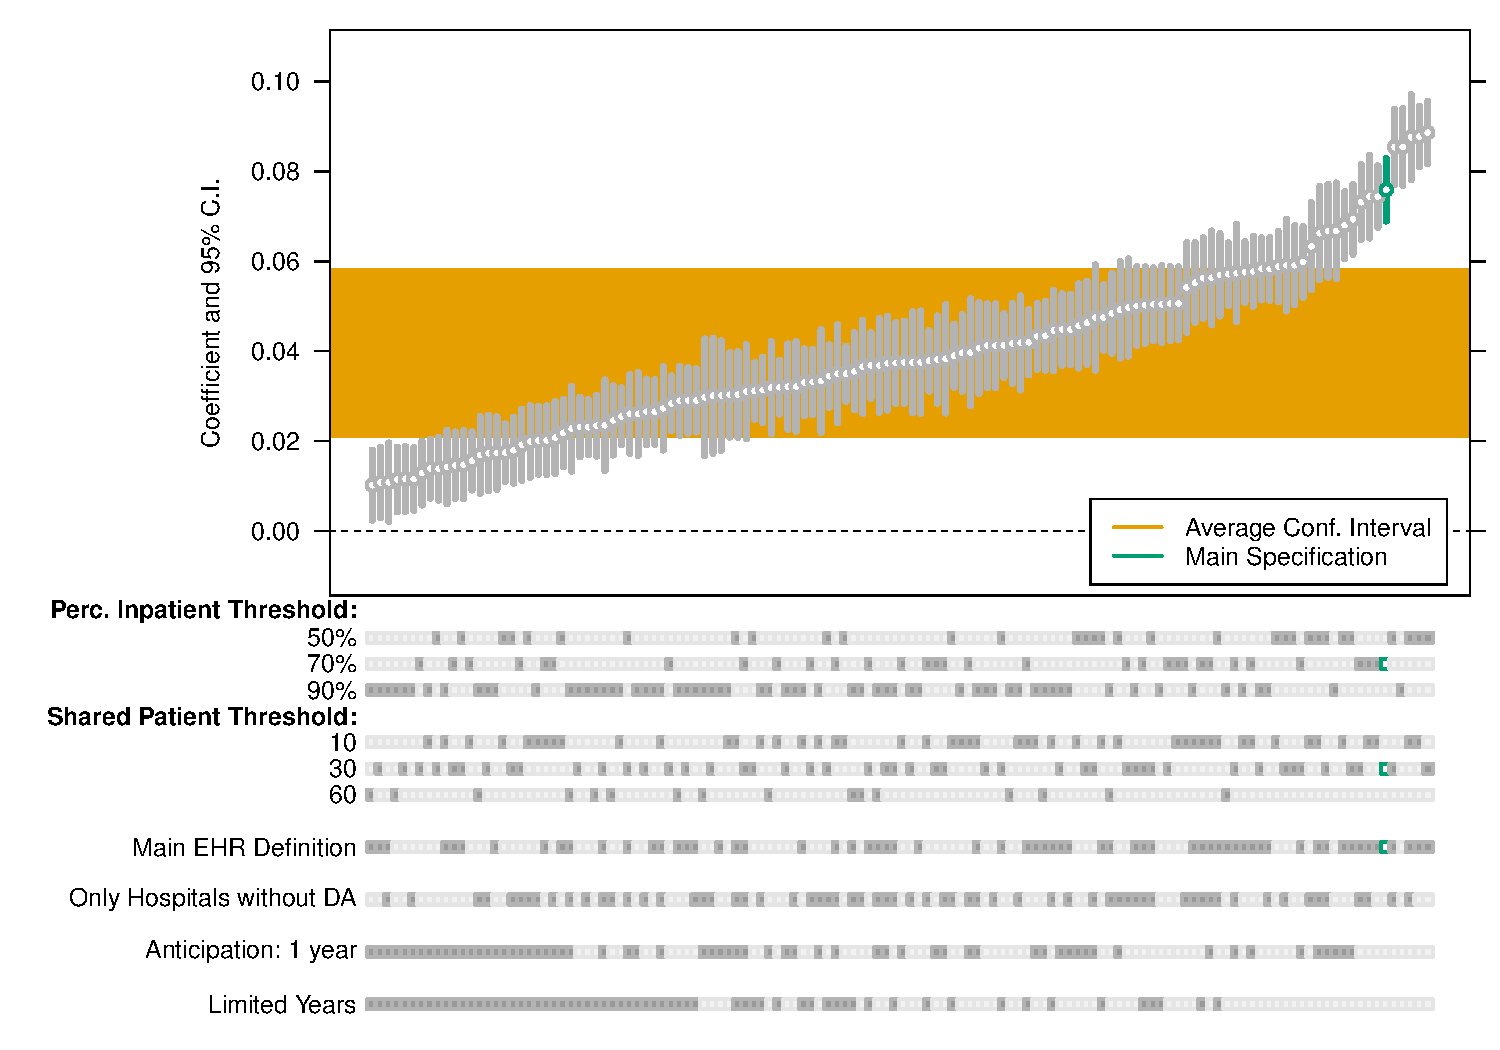
\includegraphics[scale=.45]{Objects/office_frac_chart.pdf}
    \hyperlink{Effect of EHR Exposure on Fraction of Patients in Office}{\beamerbutton{back}}
\end{frame}

\begin{frame}[noframenumbering]{Robustness: Patient Count}
\label{Robustness: Patient Count}
\centering
    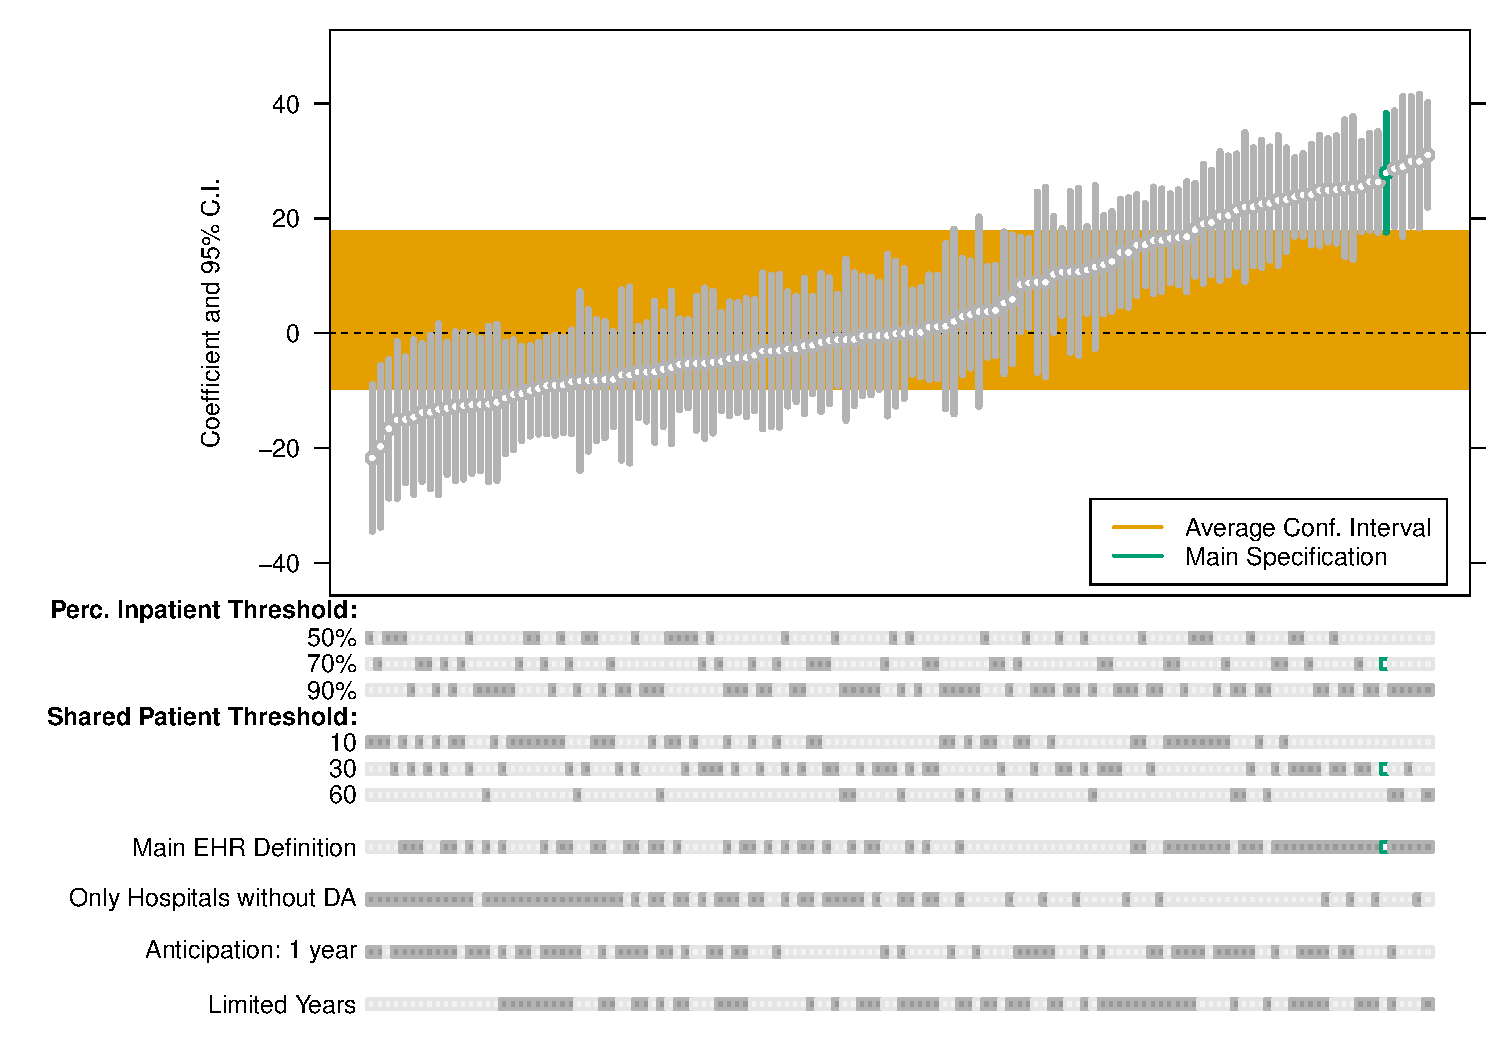
\includegraphics[scale=.45]{Objects/patient_chart.pdf}
    \hyperlink{Effect of EHR Exposure on Patient Count}{\beamerbutton{back}}
\end{frame}

\begin{frame}[noframenumbering]{Robustness: Claims per Patient}
\label{Robustness: Claims per Patient}
\centering
    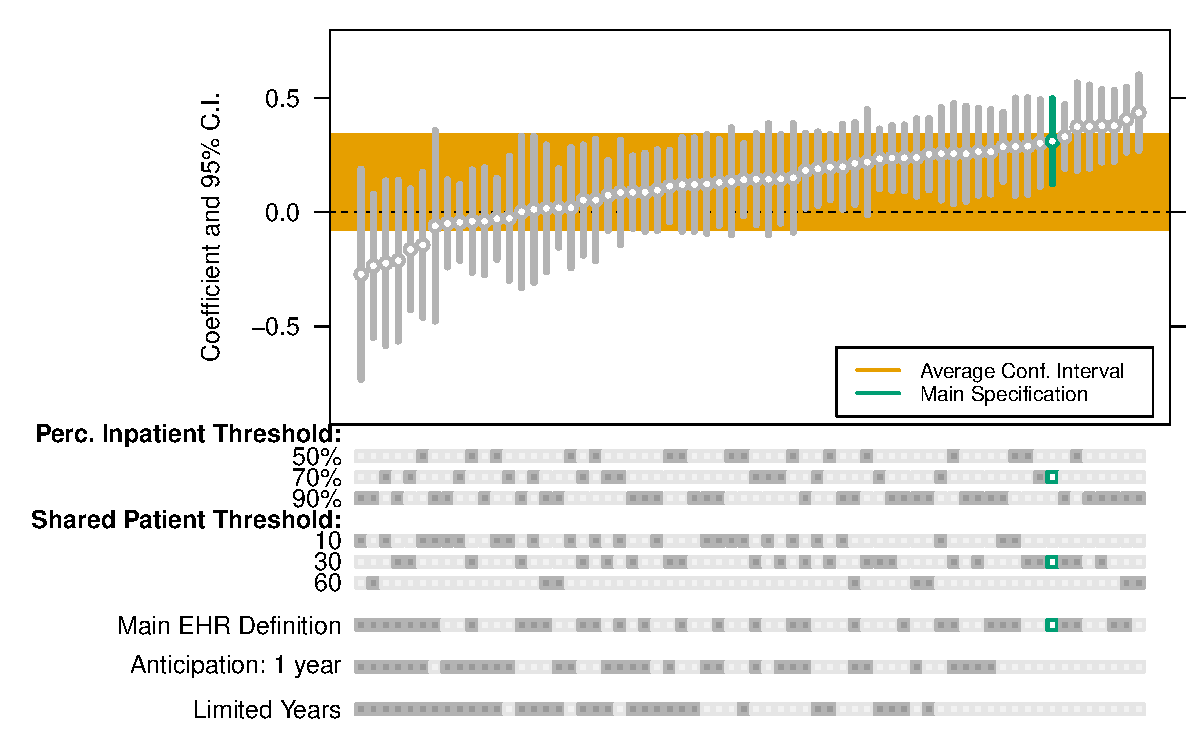
\includegraphics[scale=.45]{Objects/claim_chart.pdf}
    \hyperlink{Effect of EHR Exposure on Claims per Patient}{\beamerbutton{back}}
\end{frame}

\begin{frame}[noframenumbering]{TWFE}
\label{TWFE}
\centering
    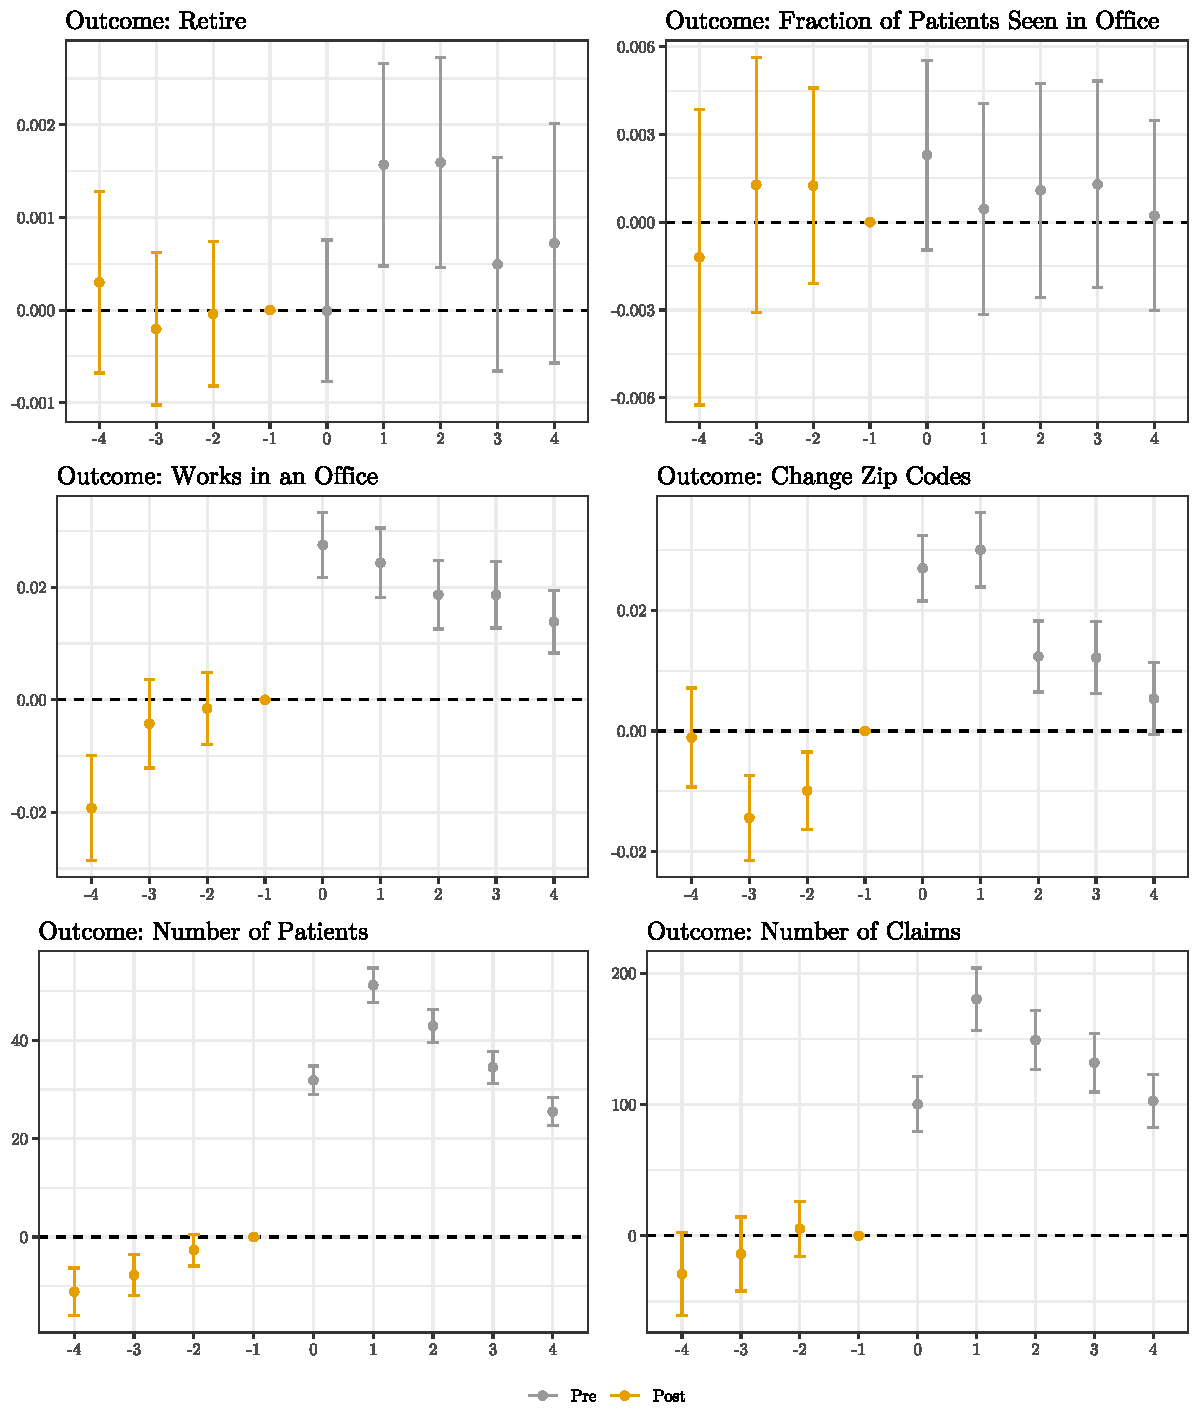
\includegraphics[scale=.3]{Objects/twfe_plot.pdf}
    \hyperlink{Robustness}{\beamerbutton{back}}
\end{frame}

\begin{frame}[noframenumbering]{Other Estimators for Staggered Treatment}
\label{Other Estimators for Staggered Treatment}
\centering
    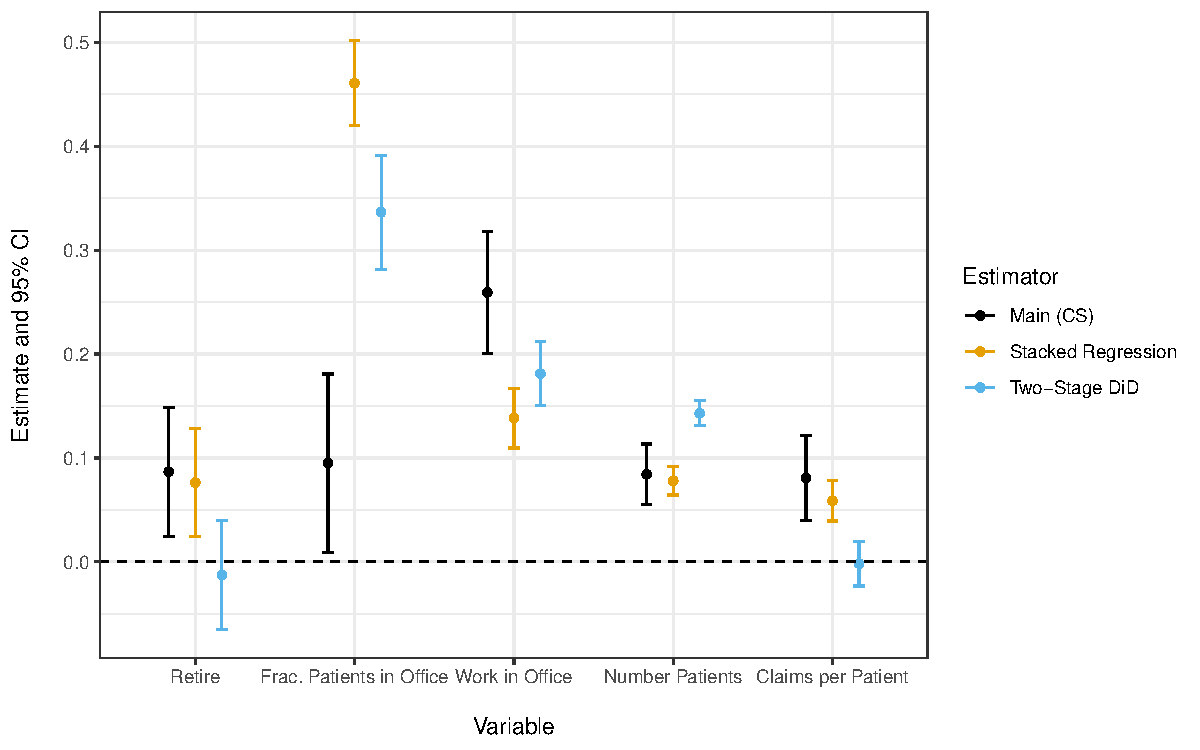
\includegraphics[scale=.45]{Objects/estimators_plot.pdf}
    \hyperlink{Robustness}{\beamerbutton{back}}
\end{frame}



\end{document}
